\documentclass[]{beamer}
% \usepackage{beamerthemelined}
\usepackage{pstricks}
\usepackage{amsfonts,amssymb,amsmath,amsthm}
\usepackage{graphicx}
\usepackage{wallpaper}
\usepackage{color}

% \setbeamertemplate{navigation symbols}{}
\beamertemplatenavigationsymbolsempty

\usetheme{Boadilla}
\usecolortheme{whale}
\setbeamertemplate{itemize items}[triangle]


\title{Cosmic Inflation}
\author{Paho Lurie-Gregg, Michael Perlin}
\date{}

\newcommand{\f}[2]{\dfrac{#1}{#2}}
\newcommand{\p}[1]{\left(#1\right)}
\renewcommand{\t}[1]{\text{#1}}
\newcommand{\abs}[1]{\left|#1\right|}

\renewcommand{\red}[1]{{\bf \color{red} #1}}
\newcommand{\fixme}[1]{\red{[#1]}}

\begin{document}

\begin{frame}
  \maketitle
  \begin{center}
    BICEP2 I: Detection of $B$-mode polarization at degree angular scales

    P.A.R. Ade, R.W. Aikin, et al.
    \vspace{1.5in}
  \end{center}

\end{frame}


\begin{frame}
  \frametitle{What}
  \begin{itemize}
  \item Period of time from $10^{-36}$ to $10^{-33}$ or $10^{-32}$ s after the
    Big Bang.
  \item Exponential expansion of space
  \end{itemize}
\end{frame}

\begin{frame}
  \frametitle{Why}
  \begin{itemize}
  \item Resolves many problems in the Big Bang theory
  \end{itemize}
\end{frame}

\begin{frame}
  \frametitle{Homogeneity}
  \begin{itemize}
  \item The horizon problem
    \begin{itemize}
    \item Universe appears homogeneous
      \begin{itemize}
      \item Without inflation, Big Bang theory does not explain how universe
        could reach equilibrium
      \end{itemize}

    \end{itemize}

  \item The smoothness problem
    \begin{itemize}
    \item Temperature fluctuations not ``yay big''
    \item Universe much smoother
    \end{itemize}

  \end{itemize}

\end{frame}


\begin{frame}
  \frametitle{The flatness problem}
  \begin{itemize}
  \item Universe has curvature equivalent to that of matter density
  \item At the Big Bang, the curvature of the universe would be sixteen orders
    of magnitude less than the density  of radiation
  \end{itemize}z

\end{frame}

\begin{frame}
  \frametitle{The magnetic monopole problem}
  \begin{itemize}
  \item Purely theoretical interest
    \begin{itemize}
    \item Many theories predict magnetic monopoles at the beginning of the
      universe
      \item Predict magnetic monopoles may exist, but in very low density
    \end{itemize}

  \end{itemize}
\end{frame}


\begin{frame}
  \frametitle{$E$ / $B$ Maps}
  \begin{figure}
    \centering
    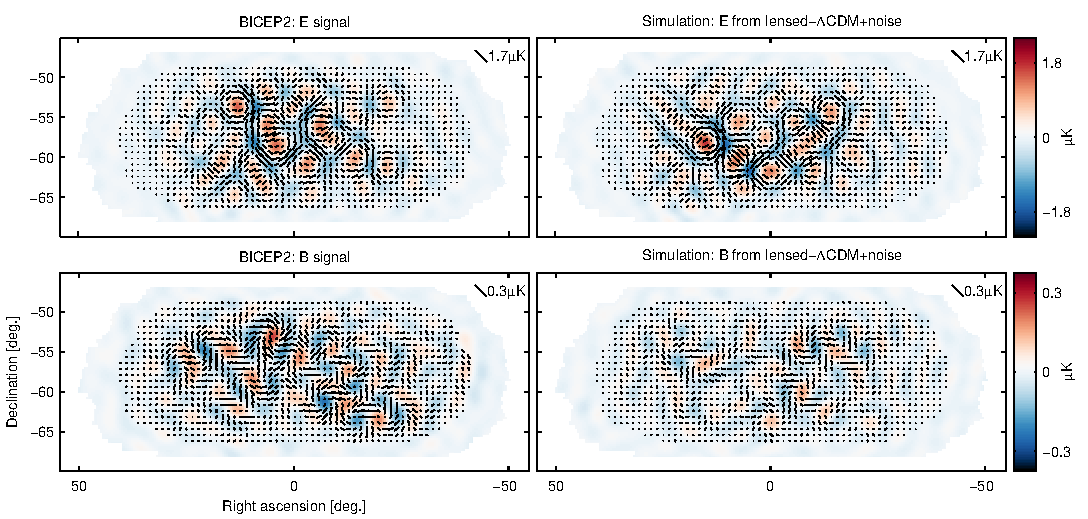
\includegraphics[width=\columnwidth]{eb_maps}
  \end{figure}
\end{frame}


\end{document}
